\documentclass[main.tex]{subfiles}

\begin{document}
\subsection{Overall Crash-Recovery Architecture}
\begin{figure}[!hbt]
	\centering
	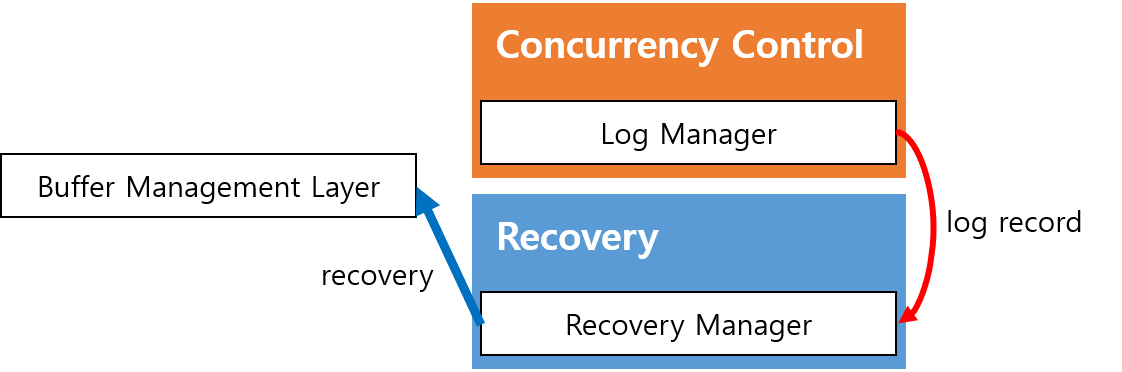
\includegraphics[width=.8\textwidth]{images/recovery/overall_architecture.png}
	\caption{Overall Design of Crash-Recovery}
	\label{rc:overall_design}
\end{figure}

위 Figure \ref{rc:overall_design}는 \texttt{Crash-Recovery}의 전반적인 구조도다.
\texttt{Crash-Recovery}는 \texttt{Concurrency Control}에서 저장한 log를 바탕으로 database file에 commit 된 데이터만 남을 수 있도록 하여 DBMS의 Atomicity와 Durability를 보장하기 위한 layer다.

\subsubsection{Recovery Manager}
\begin{table}[!htb]
	\begin{tabularx}{\textwidth}{|l|X|}
		\hline
		\textbf{File} & recovery.h recovery.cpp \\
		\hline
		\textbf{Class} & Recovery \\
		\hline
		\textbf{Purpose} & DBMS의 recovery 작업을 담당한다. \\
		\hline
	\end{tabularx}
\end{table}

\subsection{Logging}
\subsubsection{Log Structure}
\paragraph{Log Types}
Log record는 담기는 정보에 따라 다음과 같이 3가지로 분류할 수 있다.

\begin{itemize}
	\item \textbf{Base Log} $-$ log에 대한 기초적인 정보만 있는 경우\\
	종류: BEGIN, COMMIT, ROLLBACK\\
	크기: 28 bytes
	
	\item \textbf{Record Log} $-$ 복구에 관한 정보도 있는 경우\\
	종류: UPDATE\\
	크기: 288 bytes
	
	\item \textbf{Compensate Log} $-$ Record Log에 NextUndoSeq 정보도 있는 경우\\
	종류: COMPENSATE\\
	크기: 296 bytes
\end{itemize}

\paragraph{Log Structure}
Log를 표현할 때 각 log에 필요한 최소한의 공간만 사용하는 방식으로 한다면 메모리 공간 활용의 효율은 향상할 수도 있지만,
그렇게 하기 위해서 작성된 코드가 매우 복잡해지는 등의 문제가 생겼다. 따라서 공간 효율성을 희생하는 대신 코드의 퀄리티를 향상하는 방향으로 설계하였다.
따라서 Log는 다음과 같은 구조체로 표현된다.

\begin{figure}[!hbt]
	\centering
	\hspace{70px}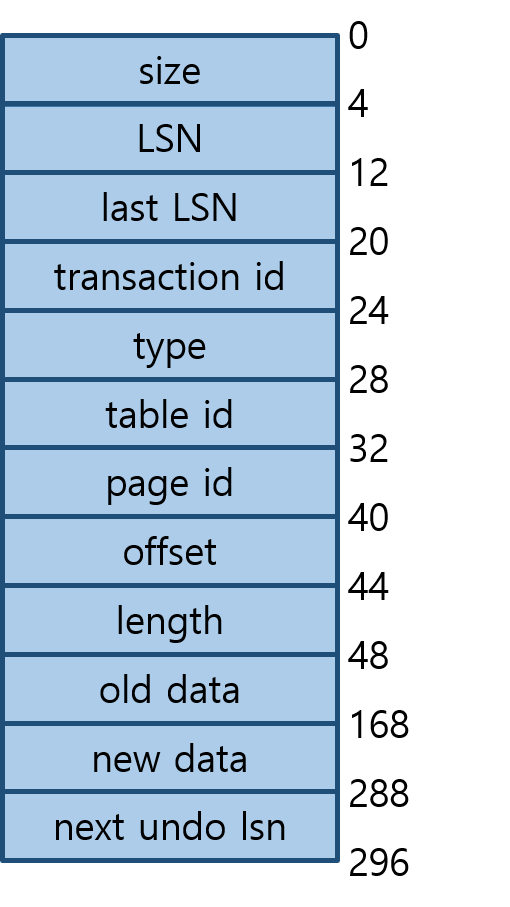
\includegraphics[width=.4\textwidth]{images/recovery/log_structure.png}
	\caption{Log Record Structure}
\end{figure}

\begin{itemize}
	\item size : log record의 크기
	\item LSN : log record의 시작 offset
	\item last LSN : 같은 transaction id를 가지는 이전 log record의 LSN
	\item transaction id : log record에 대한 transaction의 id
	\item type : log record의 type
	\item table id : data가 위치하는 table의 id
	\item page id : data가 위치하는 page의 id
	\item offset : 해당 page에서 data의 시작 offset
	\item length : data의 길이
	\item old data : Undo에서 쓰일 data의 수정 이전 image
	\item new data : Redo에서 쓰일 data의 수정 후 image
	\item next undo lsn : COMPENSATE에서 사용되는 LSN값
\end{itemize}


\newpage
\subsubsection{Log Record File}
Log record file은 \texttt{Index Management Layer} 혹은 \texttt{Transaction Manager}에서 발급한 log를 담고 있는 파일이다. Log record file의 구조는 다음과 같다.

\begin{figure}[!hbt]
	\centering
	\hspace{70px}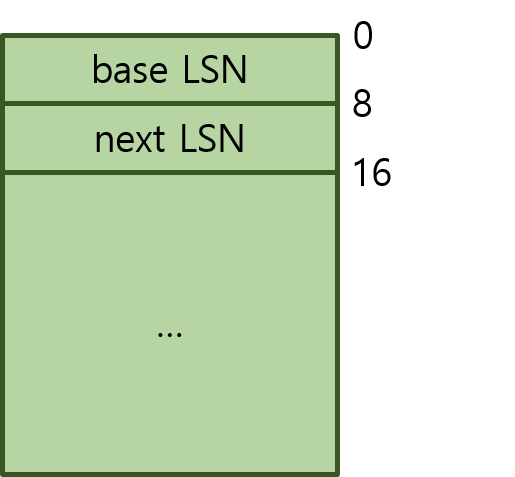
\includegraphics[width=.4\textwidth]{images/recovery/log_record_file.png}
	\caption{Log Record File Structure}
\end{figure}

다음 두 값은 log record file의 header에 해당하는 값들로 각 값의 설명은 다음과 같다.

\begin{itemize}
	\item Base LSN : log file에 있는 log record의 LSN 중 가장 작은 값
	\item Next LSN : 다음에 발급될 log의 LSN
\end{itemize}

\subsubsection{Log Management}
\paragraph{Appending Log}
Log는 \texttt{Index Management Layer}나 \texttt{Transaction Manager}에서 필요할 때 \texttt{Log Manager}에게 log 발급을 요청하면서 \texttt{Log Manager}의 buffer에 쌓이게 된다.
log의 buffer는 기본적으로 1차원 array이지만, transaction이 abort 되는 상황에 stable storage로 내려간 log를 다시 읽어와 rollback 하는데 드는 I/O 부하를 줄이기 위해
각 active transaction 별로 log의 copy를 \texttt{Log Manager} 내부에 따로 저장해둔다. 또한 이 copy는 force가 발생해도 메모리에서 지우지 않는다.
따라서 transaction의 abort가 발생할 때는 stable storage의 log record를 읽어오는 것이 아닌, 메모리에 있는 copy를 이용해 rollback을 수행한다.

\paragraph{Force}
Force란 log buffer에 있는 log record를 모두 stable storage에 저장하는 행위를 말한다.
이 과정에선 log record file의 header를 갱신하고 file의 맨 끝쪽에 log를 LSN 순서대로 덧붙이는 방식으로 저장한다.
저장이 완료되면 메모리에서 stable storage에 저장된 모든 log는 지운다.

\subsection{Recovery}
본 DBMS는 ARIES (Algorithms for Recovery and Isolation Exploiting Semantics)에 따른 three-pass recovery를 구현한다.
따라서 Analysis, Redo, Undo pass를 순차적으로 수행하며 recovery를 수행한다.

\newpage
\subsubsection{Analysis Pass}
Analysis pass에서는 전체 log record file을 읽어서 winner, loser transaction을 분류한 뒤, loser transaction에 대해서 가장 마지막 log record의 LSN을 구한다.

\begin{algorithm}
	\caption{Analysis Pass}
	
	\begin{algorithmic}
		\Function{Restart-Analysis}{}
			\State startLSN $:= \min($LogRecords$)$
			\State endLSN $:= \max($LogRecords$)$
			
			\For {lsn := startLSN to endLSN}
				\State log $:=$ LogRecords[lsn]
				
				\If {log.type is BEGIN}
					\State Xact[log.xid] $:=$ Loser
					\State LoserLastLSN[log.xid] $:= 0$
				\ElsIf {log.type $\in \left\lbrace ~ \mathrm{COMMIT} ~|~ \mathrm{ROLLBACK} ~ \right\rbrace$}
					\State Xact[log.xid] $:=$ Winner
					\State LoserLastLSN -= log.xid
				\ElsIf {log.type $\in \left\lbrace ~ \mathrm{UPDATE} ~|~ \mathrm{COMPENSATE} ~ \right\rbrace$}
					\State LoserLastLSN[log.xid] $:=$ lsn
				\EndIf
			\EndFor
		\EndFunction
	\end{algorithmic}
\end{algorithm}

\subsubsection{Redo Pass}
Redo pass에서는 전체 log record file을 읽어서 DBMS가 crash 났을 때의 상황으로 database file을 되돌린다.
이때 효율적인 redo를 위해 CONSIDER-REDO라는 개념을 사용한다.

\begin{algorithm}
	\caption{Redo Pass}
	
	\begin{algorithmic}
		\Function{Restart-Redo}{}
			\State startLSN $:= \min($LogRecords$)$
			\State endLSN $:= \max($LogRecords$)$
			
			\For {lsn := startLSN to endLSN}
				\State log $:=$ LogRecords[lsn]
				
				\If {log.type $\in \left\lbrace ~ \mathrm{UPDATE} ~|~ \mathrm{COMPENSATE} ~ \right\rbrace$ }
					\State page $:=$ BufferManager.GetPage(table id, page id)
					\If {page.PageLSN $\le$ lsn}
						\State // Consider-Redo
					\Else
						\State page.PageLSN $:=$ lsn
						\State Apply log.NewData to page
					\EndIf
				\EndIf
			\EndFor
		\EndFunction
	\end{algorithmic}
\end{algorithm}

\subsubsection{Undo Pass}
Undo pass에서는 loser transaction에 대해 undo를 수행함으로써 commit 된 record만을 database file에 남기어 atomicity를 보장한다.

\begin{algorithm}
	\caption{Undo Pass}
	
	\begin{algorithmic}
		\Function{Restart-Undo}{}
			\While {$\exists$LoserLastLSN $>0$}
				\State nextentry $:=$ $\max($LoserLastLSN$)$
				\State log $:=$ LogRecords[nextentry]
				
				\If {log.type is COMPENSATE}
					\State LoserLastLSN[log.xid] $:=$ log.NextUndoLSN
				\ElsIf {log.type is UPDATE}
					\State page $:=$ BufferManager.GetPage(table id, page id)\\
					
					\State page.PageLSN $:=$ NewLSN
					\State LogManager.AppendLog(COMPENSATE, NewLSN, log$^{-1}$, $\left( \mathrm{log}^{-1} \right)^{-1}$)
					
					\State Apply log.OldData to page
				\ElsIf {log.type is BEGIN}
					\State LoserLastLSN -= log.xid
				\EndIf
			\EndWhile
		\EndFunction
	\end{algorithmic}
\end{algorithm}

\end{document}
